\documentclass[letterpaper, 11pt]{article}
\usepackage{amsmath}
\usepackage{mathtools}
\usepackage{amssymb}
\usepackage{float}
\usepackage{inputenc}
\usepackage[left=2cm, right=2cm, top=2cm, bottom=2cm]{geometry}
\usepackage{graphicx}
\usepackage{float}
\usepackage{caption}
\usepackage{extarrows}
\usepackage{xcolor}
\usepackage{lscape}
\usepackage{pdflscape}
\usepackage{pdfpages}
\usepackage{multicol}
\usepackage{leftindex}
\usepackage{algorithm2e}
\SetKwComment{Comment}{/* }{ */}
%\RestyleAlgo{ruled}
\usepackage{mathtools}
\usepackage{hyperref}
\hypersetup{
    colorlinks=false,
    }

% Listings
\usepackage{listings}
\usepackage{color}
\definecolor{mygreen}{rgb}{0,0.6,0}
\definecolor{mygray}{rgb}{0.5,0.5,0.5}
\definecolor{mymauve}{rgb}{0.58,0,0.82}

\lstset{
  backgroundcolor=\color{white},   % choose the background color; you must add \usepackage{color} or \usepackage{xcolor}; should come as last argument
  basicstyle=\small\ttfamily,        % the size of the fonts that are used for the code
  breakatwhitespace=false,         % sets if automatic breaks should only happen at whitespace
  breaklines=true,                 % sets automatic line breaking
  captionpos=t,                    % sets the caption-position to bottom
  commentstyle=\color{mygreen},    % comment style
  deletekeywords={...},            % if you want to delete keywords from the given language
  escapeinside={\%*}{*)},          % if you want to add LaTeX within your code
  extendedchars=true,              % lets you use non-ASCII characters; for 8-bits encodings only, does not work with UTF-8
  firstnumber=1,                % start line enumeration with line 1000
  frame=false,	                   % adds a frame around the code
  keepspaces=true,                 % keeps spaces in text, useful for keeping indentation of code (possibly needs columns=flexible)
  keywordstyle=\color{blue},       % keyword style
  language=Python,                 % the language of the code
  morekeywords={*,...},            % if you want to add more keywords to the set
  numbers=none,                    % where to put the line-numbers; possible values are (none, left, right)
  numbersep=5pt,                   % how far the line-numbers are from the code
  numberstyle=\tiny\color{mygray}, % the style that is used for the line-numbers
  rulecolor=\color{black},         % if not set, the frame-color may be changed on line-breaks within not-black text (e.g. comments (green here))
  showspaces=false,                % show spaces everywhere adding particular underscores; it overrides 'showstringspaces'
  showstringspaces=false,          % underline spaces within strings only
  showtabs=false,                  % show tabs within strings adding particular underscores
  stepnumber=5,                    % the step between two line-numbers. If it's 1, each line will be numbered
  stringstyle=\color{mymauve},     % string literal style
  tabsize=4,	                   % sets default tabsize to 2 spaces
  title=\lstname                   % show the filename of files included with \lstinputlisting; also try caption instead of title
}


% NewCommands
\newcommand{\peq}{ \mathrel{+}= }
\newcommand{\muleq}{ \mathrel{*}= }
\newcommand{\sign}{ \text{sign}}
\newcommand{\bm}[1]{\begin{bmatrix} #1 \end{bmatrix}}
\newcommand{\mat}[1]{\begin{matrix} #1 \end{matrix}}
\newcommand{\lx}[2]{\leftindex #1 {#2}}
\newcommand{\norm}[1]{\left\lvert #1 \right\rvert}
\newcommand{\itbf}[1]{\textit{\textbf{#1}}}
\newcommand{\mdet}[1]{\norm{\begin{matrix} #1 \end{matrix}}}
\newcommand{\pbox}[1]{\fbox{\begin{minipage}{\textwidth} #1 \end{minipage}}}
\newcommand{\lstln}[1]{\lstinline|#1|}
\newcommand{\lr}[1]{\left( #1 \right)}
\newcommand{\lrb}[1]{\left[ #1 \right]}


\title{Notes on SCR-OBD algorithm developement}
\author{Sesha Charla}
\date{\today}


\begin{document}
\maketitle
\tableofcontents
\newpage
\
\newpage
%===============================================================================
\section{Introduction}

\itbf{Goal}:

"Developing model-based non-intrusive diagnostics for SCR-ASC that can work with commercial NO-x sensors and demonstrate the results on a real-world on-road truck data."

\bigskip

\itbf{Kaushal's work}:
\begin{itemize}
    \item Diagonstic-oriented aging models for SCR-ASC.
    \begin{itemize}
        \item Chemical Kinetics based model for SCR
        \item Non-linear look-up table for ASC
    \end{itemize}
    \item Term-by-term observer design for SCR Ammonia adsorption.
    \item Diagnosis algorithm
    \begin{itemize}
        \item Sequence of filters
        \item Residual generation for fault detection using the stochastic version of the models.
    \end{itemize}
\end{itemize}

\itbf{Available measurements}
\begin{enumerate}
    \item Engine Torque
    \item Engine Speed
    \item Diesel exhaust fluid (DEF) injection
    \item Engine-out $NO_x$.
    \item Diesel oxidation catalyst (DOC)-out $NO_x$.
    \item Tail-pipe $NO_x$. (Test cell: $NH_3$ and $N_2O$)
    \item DOC-in, DOC-out, SCR-in, SCR-out and ASC-out temperatures.
    \item Exhaust flow rate.
\end{enumerate}

\itbf{Available data}
\begin{enumerate}
    \item Road data
    \begin{itemize}
        \item Cold FTP (Federal Test Procedure)
        \item Hot FTP
        \item RMC (Ramped mode cycle)
    \end{itemize}
    \item Test Cell data
    \begin{itemize}
        \item Cold FTP (Federal Test Procedure)
        \item Hot FTP
        \item RMC (Ramped mode cycle)
    \end{itemize}

\end{enumerate}

\subsection{System Setup}
\begin{figure}[H]
    \centering
    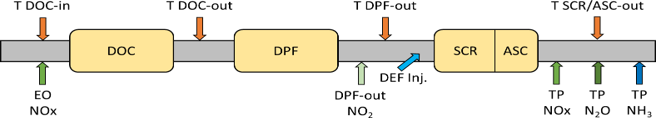
\includegraphics[width = \textwidth]{./figs/scr_system.png}
    \caption{SCR System}
\end{figure}

\subsection{Test Cell data}
From the test-cell sampling, we have
\begin{align*}
    \text{Samling time, } \qquad dt &= 0.2 \, s\\
    \text{Sampling frequency, } \quad f &= 5\, Hz
\end{align*}


\subsubsection{Test Cell data Variables}
\begin{table}[H]
\centering
\begin{tabular}{l l l c}
   \hline \hline
   Variable Name                 & Units  & Description & Variable from Model \\ \hline \hline
   LOG\_TM	                     & sec    & Time
                                          & $t$\\
   ENG\_SPD	                     & RPM    & Engine Speed
                                          &\\
   NET\_TORQ	                 & lb\_ft & Engine Torque
                                          &\\
   TEST\_CELL\_T	             & deg\_f & Test Cell Temperature
                                          &\\
   TUR\_OT\_T	                 & deg\_f & Turbine Outlet Gas Temperature
                                          &\\
   EXHAUST\_FLOW	             & kg/min & Exhaust Flow Rate
                                          & $F$\\
   V\_AIM\_TRC\_DOC\_IN	         & Deg\_C & DOC In Gas Temperature
                                          &\\
   V\_AIM\_TRC\_DOC\_OUT	     & Deg\_C & DOC Out Gas Temperature
                                          &\\
   V\_AIM\_TRC\_DPF\_OUT	     & Deg\_C & DPF Out Gas Temperature
                                          &\\
   V\_AIM\_TRC\_SCR\_OUT	     & Deg\_C & SCR/ASC Out Gas Temperature
                                          &\\
   V\_SCR\_ANR\_FDBK	         & None   & ANR (??)
                                          &\\
   V\_UIM\_FLM\_ESTUREAINJRATE	 & ml/sec & DEF (Urea Sol.) Dosing Rate
                                          & $u_2$\\
   ENG\_CW\_NOX\_FTIR\_COR\_U2	 & PPM    & Engine-Out NOx
                                          & $u_1$\\
   EXH\_CW\_NOX\_COR\_U1	     & PPM    & Tailpipe NOx
                                          & $x_1$\\
   EXH\_CW\_AMMONIA\_MEA	     & ppm    & Tailpipe NH3
                                          & $x_2$\\
   EXH\_CW\_N2O\_MEA	         & ppm    & Tailpipe N2O
                                          &\\
   ENG\_CW\_NO2\_COR\_U2	     & PPM    & DPF Outlet NO2
                                          &\\
EONOX\_COMP\_VALUE	         & ppm    & Engine-out NOx (with Corss-sensitivity)
                                      & $y_3$\\
V\_SCM\_PPM\_SCR\_OUT\_NOX	 & ppm    & SCR-out NOx  (with cross-sensitivity)                    & $y_1$\\
   \hline \hline
\end{tabular}
\caption{Test Cell Data Variables}
\end{table}

% ============================================================================
\subsubsection{Test cell data ranges}
\begin{table}[H]
\centering
\begin{tabular}{c c c c c}
\hline \hline
Variable & Units &Cold FTP & Hot FTP & RMC\\
\hline \hline
& & Degreend Data & & \\ \hline
$T$   & $^0$C & & &
\\
$F$   & $kg/min$ & & &
\\
$x_1$ & $ppm$ & & &
\\
$x_2$ & $ppm$ & & &
\\
$u_1$ & $ppm$ & & &
\\
$u_2$ & $ppm$ & & &
\\
$y_1$ & $ppm$ & & &
\\
$y_3$ & $ppm$ & & &
\\
\hline
& & Aged Data & & \\ \hline
$T$   & $^0$C & & &
\\
$F$   & $kg/min$ & & &
\\
$x_1$ & $ppm$ & & &
\\
$x_2$ & $ppm$ & & &
\\
$u_1$ & $ppm$ & & &
\\
$u_2$ & $ppm$ & & &
\\
$y_1$ & $ppm$ & & &
\\
$y_3$ & $ppm$ & & &
\\
\hline \hline
\end{tabular}
\caption{Test cell data ranges}
\end{table}


% =============================================================================

%Expt. & $F\,(kg/min)$ & $T\, (^0 C)$ & $x_1$ (ppm) & $u_1$ (ppm) & $x_2$ (ppm)
%& $u_2$ & $y_1$ & $y_3$
%\\\hline \hline
%%=======================================================================
%Aged (Cold FTP) & [0 26.64] & [28.20 262.30] & [0 558.06] & [-2.78
%760.55] & [-0.60 1.40] \\
%%=======================================================================
%Aged (Hot FTP) & [0 26.50] & [134.30 269] & [0 506.48] & [-14.40
%158.67] & [-0.60 11.10]\\
%%=======================================================================
%Aged (RMC) & [1.80 24.75] & [238.40 348.20] & [0 693.65] & [-2.24
%109.63] & [0.80 4.40]\\
%%=======================================================================
%De-greened (Cold FTP) & [0 26.72] & [25.80 253.90] & [0 609.84] &
%[-116.93 518.05] & [-0.70 1.70] \\
%%=======================================================================
%De-greened (Hot FTP) & [0 26.47] & [110.10 261.80] & [0 504.92] &
%[-17.16 110.85] & [-0.50 3.70]\\
%%=======================================================================
%De-greened (RMC) & [1.84 24.91] & [236.20 341.30] & [0 728.04] &
%[-1.30 75.61] & [0.40 5.20] \\
%

\subsection{Road data}
From the test-cell sampling, we have
\begin{align*}
    \text{Samling time, } \qquad dt &= 1 \, s\\
    \text{Sampling frequency, } \quad f &= 1 \, Hz
\end{align*}



\subsubsection{Road data variables}
\begin{table}[H]
\centering
\begin{tabular}{l l l }
\hline \hline
Model Variable & Road Data Variable &Units\\
\hline \hline
$t$   & tod & $s$
\\
$T$   & pSCRBedTemp & $^0$C
\\
$F$   & pExhMF & $kg/min$
\\
$x_1$ & & $ppm$
\\
$x_2$ & & $ppm$
\\
$u_1$ & & $ppm$
\\
$u_2$ & pUreaDosing & $ml/sec$
\\
$y_1 $ & pNOxOutppm & $ppm$
\\
$y_3 (=u_1?)$ & pNOxInppm & $ppm$
\\
\hline
\end{tabular}
\caption{Road data variables}
\end{table}


\subsubsection{Road data ranges}
\begin{table}[H]
\centering
\begin{tabular}{l l l l l l l l l l }
\hline \hline
Variable & Units & adt\_15 &adt\_17&mes\_15&mes\_18&wer\_15&wer\_20&trw\_15&trw\_16
\\
\hline \hline
$T$   & $^0$C & & & &&&&&
\\
$F$   & $kg/min$ & & & &&&&&
\\
$x_1$ & $ppm$ & & & &&&&&
\\
$x_2$ & $ppm$ & & & &&&&&
\\
$u_1$ & $ppm$ & & & &&&&&
\\
$u_2$ & $ppm$ & & & &&&&&
\\
$y_1$ & $ppm$ & & & &&&&&
\\
$y_3$ & $ppm$ & & & &&&&&
\\
\hline \hline
\end{tabular}
\caption{Road data ranges}
\end{table}


\subsection{Approach to the research problem}
Our approach is based on the presumption that the aging detection problem can be framed as a state/parameter estimation challenge with respect to the concentration dynamics of the gases involved. This gives rise to the following sub-problems:

\begin{enumerate}
\item Determining a suitable model for the system dynamics.
\item Assessing whether the available data contains sufficient information for identifying the model parameters related to the chosen system dynamics.
\item Investigating the relationship between the parameters/states and the aging factor of the catalyst.
\item Understanding the uncertainties inherent in the aforementioned processes.
\item Finally, developing and validating the aging detection algorithm.
\end{enumerate}

%===============================================================================
\newpage
\section{SCR-ASC Reactions and Dynamics}

\subsection{SCR-ASC Reactions}
Eley Rideal reaction mechanism \cite{hsieh2011development}
\cite{yuan2015diesel}, \cite{nova2014urea} is considered for the interpreting
the SCR reactions. The mechanism involves the following reactions:

\begin{align}
    NH_2 - CO - NH_2 (liquid) &\longrightarrow NH_2 - CO - NH_2^* + x H_2 O
                & &[\text{AdBlue evaporation}] \label{eqn::urea_1} \\
    NH_2 - CO - NH_2^*  &\longrightarrow  HNCO + NH_3
                & &[\text{Urea decomposition}] \label{eqn::urea_2}\\
    HNCO + H_2O &\longrightarrow NH_3 + CO_2
                & &[\text{Isocynic acid hydrolysis}] \label{eqn::urea_3}\\
    %===
    NH_3 + \theta_{free} &\longleftrightarrow NH_3(ads)
                & &[\text{Adsorption/Desorption}] \label{eqn::ads}\\
    %===
    4 NH_3 (ads) + 4 NO + O_2 &\longrightarrow 4 N_2 + 6 H_2O
                              & &[\text{Standard SCR reaction}]
                              \label{eqn::std_scr}\\
    %===
    2 NH_3 (ads) +  NO + N O_2 &\longrightarrow 2 N_2 + 3 H_2O
                              & &[\text{Fast SCR reaction}]
                              \label{eqn::fast_scr}\\
    %===
    4 NH_3 (ads) + 3N O_2 &\longrightarrow 3.5 N_2 + 6 H_2O
                              & &[\text{Slow SCR reaction}]
                              \label{eqn::slow_scr}\\
    %===
    4 NH_3 + 3 O_2 &\longrightarrow 2 N_2 + 6 H_2O
                         & &[\text{AMOX with/without ASC}]
                         \label{eqn::amox_N2}\\
    4 NH_3 + 5 O_2 &\longrightarrow 4 NO + 6 H_2 O
                         & &[\text{AMOX with/without ASC}]
                         \label{eqn::amox_NO}\\
    2 NH_3 + 2 O_2 &\longrightarrow N_2O + 3 H_2O
                         & &[\text{AMOX with/without ASC}]
                         \label{eqn::amox_N20}\\
    %==
    2 NO + O_2 &\longrightarrow 2 NO_2
                        & &[\text{NO oxidation}]
                        \label{eqn::NOX}
\end{align}


The PDE model for SCR reaction kinematics \cite{nova2014urea} is reduced to ODE model \cite{devarakonda2008adequacy} using by assuming "continuous stirred tank reactor (CSTR)" model (Control volume approach).


\subsection{General reaction kinetics}
For a stoichiometric reaction of the following form:
\begin{align*}
    a A + b B \longrightarrow c C + d D
\end{align*}
We have the reaction rate \cite{chem_kine}:
\begin{align*}
    r &= -\frac{1}{a} \frac{d [A]}{dt}
       = -\frac{1}{b} \frac{d [B]}{dt}
       = \frac{1}{c}  \frac{d [C]}{dt}
       = \frac{1}{d}  \frac{d [D]}{dt}\\
    r &= k [A]^m [B]^n\\
    \text{Where, }\quad &\\
    [\bullet] &- \text{Concentration of the reactant } \bullet\\
    k &- \text{Rate constant}\\
    m, n &- \text{Constant exponents, ($m+n$) is the order of reaction}\\
\end{align*}
In the subsequent derivations, the exponents in the rate equations are limited
to either zero or 1 $m, n \in \{0, 1\}$ (This is consistent with the assumption
that reaction rates are proportional to gas-phase concentrations from \cite{devarakonda2009model}).

The rate constant can be determined using \itbf{Arrhenius equation}:
\begin{align*}
    k &= A e^{E_a/RT}\\
    \text{Where,} \quad &\\
    A &- \text{Pre-exponential factor}\\
    E_a &- \text{Activation energy}\\
    T &- \text{Temperature}\\
    R &- \text{Universal gas constant}
\end{align*}
\subsubsection{Effects of temperature change on rate constant}
We have the Arrhenius equation:
\begin{align*}
    k &= A e^{-E_a/RT}\\
    \implies \delta k &= \delta T A \lr{\frac{E_a}{RT^2}} e^{-E_a/RT} = \delta T k \lr{\frac{E_a}{RT^2}}\\
\end{align*}
In general, $E_a$ is several orders of magnitude greater than the other
parameters. Thus, small change in temperature gets amplified as the change in
the rate-constant.

Also, we have the first-order tayer approximation for the rate-constant
variation with temperature:
\begin{align*}
    k(T_0 + \delta T) &\approx k(T_0) + \frac{E_a}{RT_0^2} k(T_0) \delta T\\
    k(\delta T) &\approx k_0 + p_0k_0 \delta T
\end{align*}
This form would be more amenable to parameter estimation despite introducing
approximation errors.



%===============================================================================
\subsection{Eley-Rideal Mechanism}
In this mechanism, proposed in 1938 by D. D. Eley and E. K. Rideal, only one of
the molecules adsorbs and the other one reacts with it directly from the gas
phase, without adsorbing ("non-thermal surface reaction") \cite{eley_rideal}.
\begin{align*}
    A(g) + S(s) &\rightleftharpoons AS(s)  \qquad (k_1, k_{-1})\\
    AS(s) + B(g) &\longrightarrow Products \qquad (k)
\end{align*}

We have the rate of the second reaction:
\begin{align*}
    r &= k C_s \theta C_B\\
    \theta &= \frac{C_{AS}}{C_S}
\end{align*}
Thus,
\begin{align*}
    \frac{d C_{AS}}{dt} &= k_1 C_A C_S (1-\theta) - k_{-1} \theta C_S - k C_S \theta C_B\\
    \text{At equilibrium}:\qquad &\\
    \frac{d C_{AS}}{dt} &= 0
    \implies \theta = \frac{k_1 C_A C_S}{k_1 C_A C_s + k_{-1}C_S + k C_s C_B}
\end{align*}
Based on the rate of individual reactions, we have the following
simplifications:
\begin{enumerate}
    \item If the limiting step is adsorption/desorption:
    \begin{align*}
        \implies k C_B &\gg k_1 C_A, k_{-1}\\
        \implies \theta &= 1 \implies r = k C_S C_B
    \end{align*}

    \item If the limiting step is the reaction:
    \begin{align*}
        \implies k C_B &\ll k_1 C_A, k_{-1}\\
        \implies \theta &= \frac{k_1 C_A C_S}{k_1 C_A C_S + k_{-1}C_S}
                        = \frac{K_{ad} C_A}{K_{ad}C_A + 1} \qquad
        \text{where, } K_{ad} = \frac{k_1}{k_{-1}} \qquad
        [\text{Langmuir's Isotherm}]\\
        \implies r &= k C_S C_B \frac{K_{ad} C_A}{K_{ad}C_A + 1}
    \end{align*}
The above expression can be further simplified based on the relative
concentrations of A and B:
\begin{enumerate}
    \item High concentrations of A, $(C_A \gg C_B)$:
    \begin{align*}
        \implies r &= k C_S C_B
    \end{align*}
    The order of the reaction is zero w.r.t A.
    \item Low concentrations of A, $(C_A \ll C_B)$:
    \begin{align*}
        r &= k C_S K_{ad} C_A C_B = k_r C_S C_A C_B
    \end{align*}
\end{enumerate}
\end{enumerate}

\itbf{Note}: Arrhenius equation can be used to model the temperature dependence
of the adsorption and desorption rate constants (thermal-desroption).

% ==============================================================================

% ==============================================================================
\subsection{Reaction Rates}
\itbf{Assumptions:}
\begin{enumerate}
\item The reaction rates are only functions of gas-phase concentrations of $NO$,
$NH_3$, the adsorbed Ammonia and the available adsorption sites.

\item The concentration rates are converted into molar-rate so that the
mass balance in control volume approach (CSTR) can be performed. For gaseous reactants:
$$ M_g = C_g V \implies R_i = V r_i $$
The number of moles of the adsorbant is directly considered instead of their
surface concentrations.

\item A lower order Tayler approximation is assumed to model the temperature
effects in rate constant.
\end{enumerate}

\begin{enumerate}
\item Standard SCR Reaction (\ref{eqn::std_scr}):
\begin{align*}
    R_1 &= k_1 V C_{NO} M_{NH_3} = k_1V C_{NO} \Theta \theta\\
    k_1 &= A_1 e^{\frac{-E_1}{RT}}
\end{align*}

\item Ammonia Oxidation (\ref{eqn::amox_N2}):
\begin{align*}
    R_3 &= k_3 M_{NH_3} = k_3 \Theta \theta\\
    k_3 &= A_3 e^{\frac{-E_3}{RT}}
\end{align*}

\item Ammonia Adsorption/Desorption (\ref{eqn::ads}):
\begin{enumerate}
\item Forward:
\begin{align*}
    R_{4F} &= k_{4F} V C_{NH_3} \lr{\Theta - M_{NH_3}}
            = k_{4F} V C_{NH_3} \Theta \lr{1 - \theta}\\
    k_{4F} &= A_{4F} e^{\frac{-E_{4F}}{RT}}
\end{align*}

\item Reverse:
\begin{align*}
    R_{4R} &= k_{4R} M_{NH_3}
            = k_{4R} \Theta \theta \\
    k_{4R} &= A_{4R} e^{\frac{-E_{4R}}{RT}}
\end{align*}
\end{enumerate}
\end{enumerate}

Where,
\begin{align*}
    \theta &- NH_3 \text{ storage capacity fraction in SCR } = \frac{\text{Moles of $NH_3$ adsorbed} (M_{NH_3})}{\text{Total moles of $NH_3$ that can be adsorbed} (\Theta)}\\
    \Theta &- \text{Ammonia storage capacity} (moles)\\
    \Theta &= S_1 e^{S_2 T} \qquad \qquad \begin{matrix*}[l]
                S_1, S_2 &-& \text{Aging parameters of the catalyst (positve constants)}
            \end{matrix*}\\
    E_i &- \text{Activation Energy of $i^{th}$ reaction}\\
    k_i &- \text{Pre-exponential factor}\\
    R &- \text{Universal gas constant}\\
    T &- \text{Temperature}\\
    C_{\{\bullet\}} &- \text{Concentration} \lr{mol/m^3}\\
    V &- \text{Volume of the exhaust gas in the substrate\cite{devarakonda2009model}} \lr{m^3}\\
    V_e &= \epsilon A_c L_{cat}\\
        &\begin{matrix*}[l]
        A_c &-& \text{Open frontal area of the catalyst}\\
        L_{cat} &-& \text{Length of the catalyst}\\
        \epsilon &-& \text{Void fraction}
        \end{matrix*}\\
    A_c &- \text{Area of the catalyst}
\end{align*}

%===============================================================================
\newpage
\section{Ammonia input (Urea Dosing) dynamics}
The actual input to the system is urea [from AdBlue ($32.5\%$ aqueous urea
solution)] injection that converted to ammonia (through reactions:
(\ref{eqn::urea_1}), (\ref{eqn::urea_2}) and (\ref{eqn::urea_3})). This can be modelled by the following equation \cite{nova2014urea}:
\begin{align*}
    \dot C_{NH_3, in} &= - \frac{1}{\tau} C_{NH_3, in} + 2 \frac{1}{\tau} \frac{ \eta u_{inj}}{N_{urea} F}\\
    \text{where, } \quad &\\
    \tau &- \text{Time constant}\\
    u_{inj} &- \text{Mass injection rate of the AdBlue solution}\\
    \eta &- \text{Mass fraction of urea in the solution}\\
    N_{urea} &- \text{Atomic number of urea}\\
    F &- \text{Exhaust flow rate of the catalyst } m^3/s
\end{align*}

\itbf{Assumptions}:
\begin{enumerate}
    \item The above model assumes that the evaporation of the urea-solutions
        (reaction: \ref{eqn::urea_1}) is a significantly slower process as
        compared to it's decomposition into ammonia. Thus, the reaction
        kinetics are neglected and the eveporation is considerd are a first
        order process w.r.t the vapour pressure of the ammonia.
    \item The injection dynamics are completely decoupled from that of other
        states.
    \item Further, it is observed that Urea is completely converted to Ammonia
        at the very upstream part of the SCR catalyst
        \cite{hsieh2011development}.
\end{enumerate}

Reparametrizing the above equation, let,
\begin{align*}
    x_4 &= C_{NH_3, in} \qquad b_u = 2 \frac{ \eta}{N_{urea}} \qquad \omega_u = \frac{1}{\tau}\\
    u_2 &= u_{inj}
\end{align*}

\begin{equation}{\label{eqn::urea_inj}}
    \dot x_4 = - \omega_u x_4 +   \frac{\omega_u b_u}{F} u_{2}
\end{equation}

%===============================================================================
\newpage
\section{3 state dynamic model}
\itbf{Assumptions }:

The following are the additional assumptions along with the assumptions of
4-state model that are used to arrive at the three-state dynamic model\cite{devarakonda2009model}:
\begin{enumerate}
    \item Only the standard SCR reaction is considered.
    \item All $NO_x$ in the exhaust gas is assumed to be $NO$.
    \begin{itemize}
        \item The commercially available $NO_x$ sensor (Horiba gas analyzer \cite{nova2014urea}) cannot differentiate between $NO$ and $NO_2$.
    \end{itemize}
    \item Slow SCR reaction is neglected.
    \begin{itemize}
        \item The flow rate of the exhaust would ensure that the not a significant concentration of tail-pipe exhaust components are due to the slow SCR reaction \cite{nova2014urea}.
    \end{itemize}
    \item Mass transfer is neglected. That means the chemical kinetics in the catalyst are reaction controlled.
    \begin{itemize}
        \item The standard SCR reaction rate is faster than the flow rate of the exhaust fluids.
    \end{itemize}
    \item Nitrogen selectivity for ammonia oxidation is $100\%$.
    \begin{itemize}
        \item This assumption is relaxed by including algebraic relationship between selectivity and the temperature (ASC model \cite{jain2023diagnostics}).
    \end{itemize}
    \item Reaction rates are assumed to be a function of the gas phase concentration of $NO_x$ and ammonia storage.
\end{enumerate}

\itbf{Dynamic Model Derivation}:

We have the mass (moles of reactants in/out) balance from the CSTR assumption:
\begin{align*}
    \bm{V \dot C_{NO}\\ V \dot C_{NH_3} \\ \dot M_{NH_3} } &=
    \bm{
        -R_1 - F C_{NO}\\
        -R_{4F} + R_{4R} - F C_{NH_3}\\
        R_{4F} - R_{4R} - R_1 - R_3
    } +
    F \bm{1 & 0 \\ 0 & 1 \\ 0 & 0} \bm{ C_{NO, in} \\ C_{NH_3, in}}\\
    % ===
    \text{Let, } b_v &= \frac{1}{V}\\
\end{align*}
\begin{equation} \label{eqn::mass_balance}
    %===
    \bm{\dot C_{NO} \\  \dot C_{NH_3} \\ \dot M_{NH_3} } = \frac{1}{V}
    \bm{
        -R_1 - F C_{NO}\\
        -R_{4F} + R_{4R} - F C_{NH_3}\\
        R_{4F} - R_{4R} - R_1 - R_3
    } +
    Fb_v \bm{1 & 0 \\ 0 & 1 \\ 0 & 0} \bm{ C_{NO, in} \\ C_{NH_3, in}}\\
    %===
\end{equation}

%===============================================================================
\subsection{Dynamic Model with storage ratio $(\theta)$ as state}
Let,
\begin{align*}
    \bm{x_1 \\ x_2 \\ x_3} = \bm{C_{NO} \\ C_{NH_3} \\ \theta} \qquad &
    \bm{u_1 \\ u_2 } = \bm{C_{NO, in} \\ C_{NH_3, in}}
\end{align*}
Rewriting eqn.~\ref{eqn::mass_balance}:
\begin{equation}\label{eqn::3_state_theta}
    \bm{\dot x_1 \\ \dot x_2 \\ \dot x_3} =
    \bm{[k_1 \Theta] x_1 x_3 - b_v F x_1 \\
        -[k_{4F} \Theta] x_2 (1-x_3) + [k_{4R} V^{-1} \Theta] x_3 - b_v F x_2 \\
        +[k_{4F}V] x_2 (1-x_3) - [k_{4R}] x_3 - [k_1 V] x_1 x_3 - [k_3 ] x_3} +
    b_v F \bm{1 & 0 \\ 0 & 1 \\ 0 & 0} \bm{u_1 \\ u_2}\\
\end{equation}

The following parameters are defined for convenience, based on the coefficients
of product of states and individual states in each of the equations:
\begin{align*}
    \text{Coefficients of product of states:} &\qquad& \text{Coefficients of states:}\\
    \mat{   & x_1    & x_2      & x_3    \\
        x_1 &        &          & f_{13} \\
        x_2 &        &          & f_{23} \\
        x_3 & f_{31} & f_{32}   &}
    &\qquad &
    \mat{    & x_1    & x_2      & x_3    \\
        x_1  & g_1    &          &        \\
        x_2  &        & g_{2}    & g_{23} \\
        x_3  &        & g_{32}   & g_{3}}
\end{align*}
\begin{align*}
    \mat{
    \\f_{13} &=& k_1 \Theta
    \\f_{23} &=& k_{4F} \Theta
    \\f_{32} &=& k_{4F} V
    \\f_{31} &=& k_1 V
    }
    \qquad \qquad
    \mat{
    \\ g_1    &=& b_v F
    \\ g_2    &=& b_v F + k_{4F} \Theta
    \\ g_{3}  &=& [k_{4R}+k_3]
    \\ g_{23} &=& k_{4R} V^{-1} \Theta
    \\ g_{32} &=& k_{4F} V
    }
\end{align*}
\begin{equation}\label{eqn::parm_model_theta}
     \bm{\dot x_1 \\
        \dot x_2\\
        \dot x_3\\
        } =
    \bm{
        -f_{13} x_1 x_3
        -g_1 x_1
        \\
        %===
        -g_2 x_2
        + f_{23} x_2 x_3
        + g_{23} x_3
        \\
        %===
        -f_{32} x_2 x_3
        -g_3 x_3
        -f_{31} x_1 x_3
        + g_{32} x_2
    }
    + b_v F \bm{u_1 \\ u_2 \\ 0}
\end{equation}

\itbf{Note}: Some $f_{\bullet}\,'s, g_{\bullet}\,'s$ are algebraically related.

\subsubsection{Small Perturbation model}
We have the small-perturbation model from eqn.~\ref{eqn::parm_model_theta}:
\begin{equation}\label{eqn::sml_ptrb_theta}
     \bm{\delta \dot x_1 \\
        \delta \dot x_2\\
        \delta \dot x_3\\
        } =
    \bm{
        -\lr{g_1 + f_{12} x_{30}} &
        0                                  &
        -f_{13} x_{10}
        \\
        %===
        0 &
        -\lr{g_2 - f_{23} x_{30}} &
        \lr{f_{23} x_{20}+ g_{23}}
        \\
        %===
        -f_{31} x_{30}  &
        g_{32} - f_{32} x_{30}&
        -f_{32} x_{20} - g_3 - f_{31} x_{10}
    }
    \bm{\delta x_1\\
        \delta x_2\\
        \delta x_3\\
        }
    + b_v F \bm{\delta u_1 \\ \delta u_2 \\ 0}
\end{equation}


%===============================================================================

\subsection{Dynamic Model with molar storage ratio $(M_{NH_3})$ as state}
Let,
\begin{align*}
    \bm{x_1 \\ x_2 \\ x_3} = \bm{C_{NO} \\ C_{NH_3} \\ M_{NH_3}} \qquad &
    \bm{u_1 \\ u_2 } = \bm{C_{NO, in} \\ C_{NH_3, in}}
\end{align*}
Rewriting eqn.~\ref{eqn::mass_balance}:
\begin{equation}\label{eqn::3_state_M}
    \bm{\dot x_1 \\ \dot x_2 \\ \dot x_3} =
    \bm{k_1 x_1 x_3 - b_v F x_1 \\
        -k_{4F}  x_2 (\Theta-x_3) + [k_{4R} V^{-1}] x_3 - b_vF x_2 \\
        +[k_{4F}V] x_2 (\Theta-x_3) - [k_{4R}] x_3 - [k_1V] x_1 x_3 - k_3 x_3} +
    b_v F \bm{1 & 0 \\ 0 & 1 \\ 0 & 0} \bm{u_1 \\ u_2}\\
\end{equation}

The following parameters are defined for convenience, based on the coefficients
of product of states and individual states in each of the equations:
\begin{align*}
    \text{Coefficients of product of states:} &\qquad& \text{Coefficients of states:}\\
    \mat{   & x_1    & x_2      & x_3    \\
        x_1 &        &          & f_{13} \\
        x_2 &        &          & f_{23} \\
        x_3 & f_{31} & f_{32}   &}
    &\qquad &
    \mat{    & x_1    & x_2      & x_3    \\
        x_1  & g_1    &          &        \\
        x_2  &        & g_{2}    & g_{23} \\
        x_3  &        & g_{32}   & g_{3}}
\end{align*}
\begin{align*}
    \mat{
    \\f_{13} &=& k_1
    \\f_{23} &=& k_{4F}
    \\f_{32} &=& k_{4F} \Theta
    \\f_{31} &=& k_1 V
    }
    \qquad \qquad
    \mat{
    \\ g_1    &=& b_v F
    \\ g_2    &=& b_v F + k_{4F} \Theta
    \\ g_{3}  &=& k_{4R}+k_3
    \\ g_{23} &=& k_{4R} V^{-1}
    \\ g_{32} &=& k_{4F} V \Theta
    }
\end{align*}
\begin{equation}\label{eqn::parm_model_M}
     \bm{\dot x_1 \\
        \dot x_2\\
        \dot x_3\\
        } =
    \bm{
        -f_{12} x_1 x_3
        -g_1 x_1
        \\
        %===
        -g_2 x_2
        + f_{23} x_2 x_3
        + g_{23} x_3
        \\
        %===
        -f_{32} x_2 x_3
        -g_3 x_3
        -f_{31} x_1 x_3
        + g_{32} x_2
    }
    + b_v F \bm{u_1 \\ u_2 \\ 0}
\end{equation}

\itbf{Note}: Some $f_{\bullet}'s, g_{\bullet}'s$ are algebraically related.

\subsubsection{Small Perturbation model}
We have the small-perturbation model from eqn.~\ref{eqn::parm_model_M}:
\begin{equation}\label{eqn::sml_ptrb_M}
     \bm{\delta \dot x_1 \\
        \delta \dot x_2\\
        \delta \dot x_3\\
        } =
    \bm{
        -\lr{g_1 + f_{12} x_{30}} &
        0                                  &
        -f_{12} x_{10}
        \\
        %===
        0 &
        -\lr{g_2 - f_{23} x_{30}} &
        \lr{f_{23} x_{20}+ g_{23}}
        \\
        %===
        -f_{31} x_{30}  &
        g_{32} - f_{32} x_{30}&
        -f_{32} x_{20} - g_3 - f_{31} x_{10}
    }
    \bm{\delta x_1\\
        \delta x_2\\
        \delta x_3\\
        }
    + b_v F \bm{\delta u_1 \\ \delta u_2 \\ 0}
\end{equation}

%===============================================================================
\subsection{Parametrization w.r.t the choice of $x_3$}

\begin{figure}[H]
 \begin{align*}
    \mat{
    \\f_{13} &=& k_1 \Theta
    \\f_{23} &=& k_{4F} \Theta
    \\f_{32} &=& k_{4F} V
    \\f_{31} &=& k_1 V
    }
    \qquad \qquad
    \mat{
    \\ g_1    &=& b
    \\ g_2    &=& b + k_{4F} \Theta
    \\ g_{3}  &=& [k_{4R}+k_3]
    \\ g_{23} &=& k_{4R} V^{-1} \Theta
    \\ g_{32} &=& k_{4F} V
    }
\end{align*}
 \caption*{Parametrization if $x_3 = \theta_{NH_3}$}
\end{figure}
\begin{figure}[H]
\begin{align*}
    \mat{
    \\f_{13} &=& k_1
    \\f_{23} &=& k_{4F}
    \\f_{32} &=& k_{4F} \Theta
    \\f_{31} &=& k_1 V
    }
    \qquad \qquad
    \mat{
    \\ g_1    &=& b
    \\ g_2    &=& b + k_{4F} \Theta
    \\ g_{3}  &=& k_{4R}+k_3
    \\ g_{23} &=& k_{4R} V^{-1}
    \\ g_{32} &=& k_{4F} V \Theta
    }
\end{align*}
\caption*{Parametrization if $x_3 = M_{NH_3}$}
\end{figure}

In the second parametrization $\Theta$ is only coefficient of $k_{4F}$. This can
reduce the variance of estimation.

% ==============================================================================
\subsection{Indroducing uread-dosing dyanmics}
Using the parameetric model with $x_3 = M_{NH_3}$ and introducing urea dosing
dyanmics from eqn.~\ref{eqn::urea_inj}. ($u_2$ becomes $x_4$.)
\begin{align*}
    \bm{x_1 \\ x_2 \\ x_3 \\ x_4} = \bm{C_{NO} \\ C_{NH_3} \\ M_{NH_3} \\ C_{NH_3, in}} \qquad &
    \bm{u_1 \\ u_2 } = \bm{C_{NO, in} \\ u_{inj}}
\end{align*}
\begin{align*}
    \mat{
    \\f_{13} &=& k_1
    \\f_{23} &=& k_{4F}
    \\f_{32} &=& k_{4F} \Theta
    \\f_{31} &=& k_1 V
    \\f_{24} &=& b_v F
    }
    \qquad
    \mat{
    \\ g_1    &=& b_v F
    \\ g_2    &=& b_v F + k_{4F} \Theta
    \\ g_{3}  &=& k_{4R}+k_3
    \\ g_{23} &=& k_{4R} V^{-1}
    \\ g_{32} &=& k_{4F} V \Theta
    \\ g_4 &=& \omega_u
    }
    \qquad
    \mat{
        b_{11} &=& b_v F
        \\
        b_{42} &=& \frac{\omega_u b_u}{F}
    }
\end{align*}
\begin{equation}{\label{eqn::full_nonlinear}}
     \bm{\dot x_1 \\
        \dot x_2\\
        \dot x_3\\
        \dot x_4} =
    \bm{
        -f_{13} x_1 x_3
        -g_1 x_1
        \\
        %===
        -g_2 x_2
        + f_{23} x_2 x_3
        + g_{23} x_3
        + f_{24} x_4
        \\
        %===
        -f_{32} x_2 x_3
        -g_3 x_3
        -f_{31} x_1 x_3
        + g_{32} x_2
        \\
        %===
        -g_4 x_4
    }
    + \bm{b_{11} & 0\\
          0     & 0\\
          0     & 0\\
          0     & b_{42}  }\bm{u_1 \\ u_2 }
\end{equation}

\subsection{Linear perturbation model}


%===============================================================================
\newpage
\section{Catalyst molar storage capacity model}
The variation of storage capacity of the catalyst ($\Theta$) with temperature is
modelled using an exponential curve fit in \cite{hsieh2011development} (2011)
from the available experimental data from
\cite{willems2007closed}, \cite{ciardelli2004scr} and \cite{joo2008study}.  The
results from \cite{schmieg2012thermal} (2012) show a similar trend.

\begin{align*}
    \Theta &= S_1 e^{-S_2 T}
\end{align*}

The parameters $S_1$ and $S_2$ change with age effecting the storage capacity at
a given temperature.

\begin{figure}[H]
    \begin{minipage}{0.49\textwidth}
        \begin{figure}[H]
            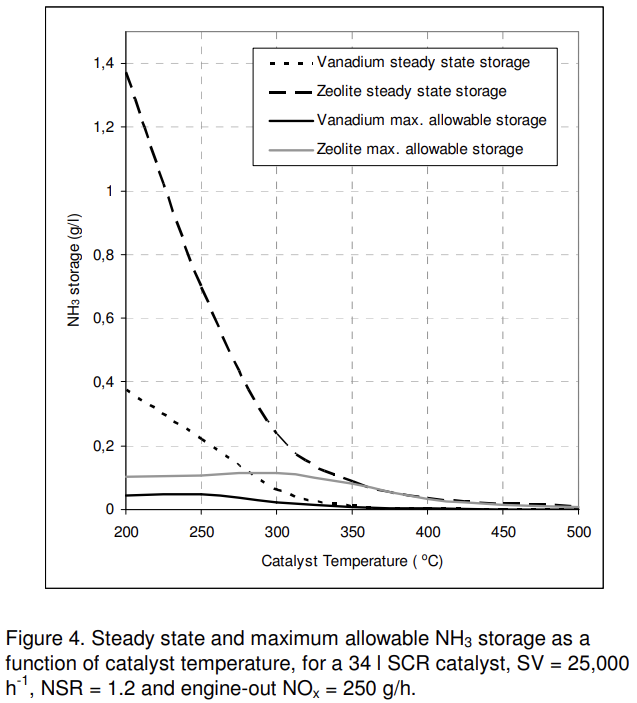
\includegraphics[width = 0.8\textwidth]{./figs/storage_capacity/sae.png}
            \caption*{Results from \cite{willems2007closed}}
        \end{figure}
    \end{minipage}
    \begin{minipage}{0.49\textwidth}
        \begin{figure}[H]
            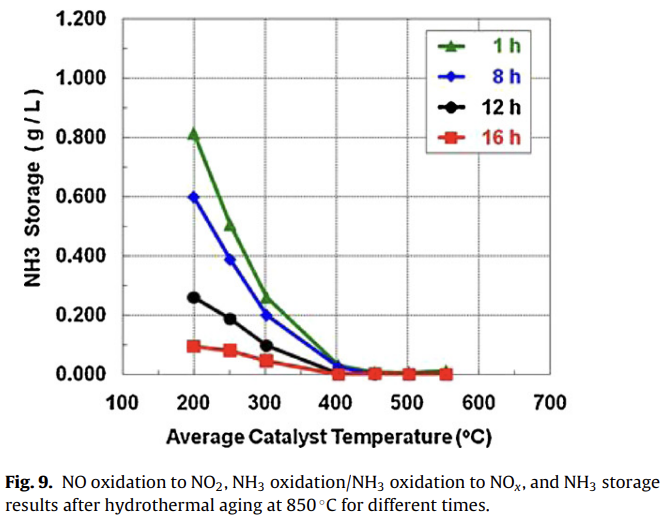
\includegraphics[width = \textwidth]{./figs/storage_capacity/th1.png}
            \caption*{Results from \cite{schmieg2012thermal}}
        \end{figure}
    \end{minipage}
    \begin{minipage}{0.49\textwidth}
        \begin{figure}[H]
            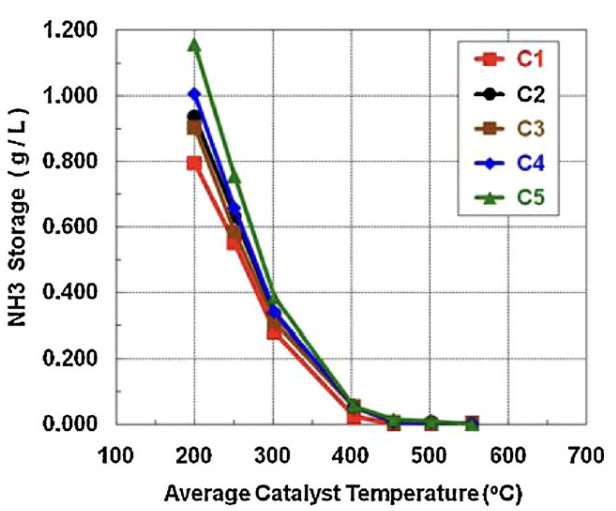
\includegraphics[width = \textwidth]{./figs/storage_capacity/th_2.png}
            \caption*{Results from \cite{schmieg2012thermal}}
        \end{figure}
    \end{minipage}
    \begin{minipage}{0.49\textwidth}
        \begin{figure}[H]
            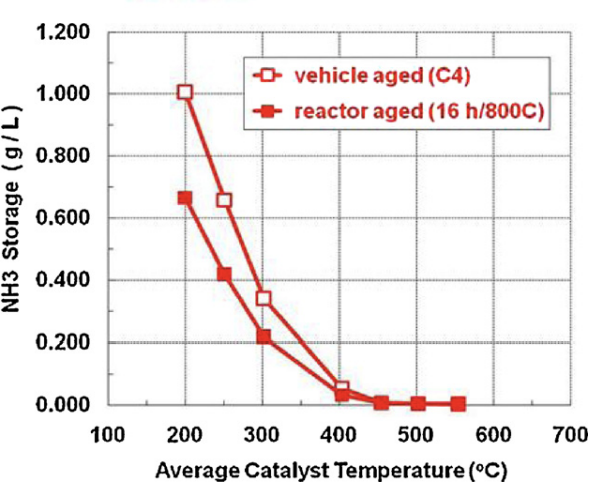
\includegraphics[width = \textwidth]{./figs/storage_capacity/th_3.png}
            \caption*{Results from \cite{schmieg2012thermal}}
        \end{figure}
    \end{minipage}
    \caption{Temperature effects of catalyst storage capacity}
\end{figure}


\subsection{Catalyst aging factor}

\itbf{Assumption}: The aged catalyst results in small changes in
$S_1, S_2$.

The above assumption is valid if the catalyst's operating range is limited to a
small range of storage capacity.

Using small perturbation,
\begin{align*}
    \delta \Theta &= \lr{\frac{\delta S_1}{S_1} - \delta S_2T} S_1 e^{-S_2 T}\\
    \implies \Theta_{aged} &= \Theta + \delta \Theta = \lr{1 + \frac{\delta S_1}{S_1} - \delta S_2T} S_1 e^{-S_2 T}
\end{align*}

Let,
\begin{align*}
    a(T) &= 1 + \frac{\delta S_1}{S_1} - \delta S_2T = a_1 + a_2 T
\end{align*}

Thus, $a$ is the factor by which the storage capacity is reduced due to the
catalyst's aging. Hence, for optimal performance:
\begin{align*}
    a > a_{min} \quad \forall T \in [T_{min}, T_{max}]
\end{align*}

\itbf{Note}: The above definition is consistent with that of the literature
\cite{ma2017observer}. The major difference lies in its derivation and
assumptions. Also, \cite{ma2017observer} considers aging factor as temperature
independent fraction and has no minimum value for classifying the catalyst as aged.

Consequently, \itbf{the catalyst aging detection problem becomes estimating the
aging factor and testing if it is bellow $a_{min}$ in presence of
uncertainties}.


\subsubsection{Aging factor estimation problem formulation}
Given the simplified non-linear concentration dynamics for SCR-ASC
reactions with internal dynamics and sensor corss-sensitivity
\ref{eqn::ctrl_state}. Estimate the total molar
Ammonia storage capacity of the catalyst [$\Theta(t, T)$]. Then,
\begin{align*}
    a(t, T) &= \frac{\Theta(t, T)}{\Theta(0, T)} = a_1 + a_2 T
\end{align*}


\itbf{No fault condition:}
$$ a(t, T) > a_{min} \quad \forall T \in [T_{min}, T_{max}], \: t > 0$$

\bigskip

We have the following high-level steps in fault-diagnosis:
\begin{enumerate}
    \item Estimate cross-sensitivity factor $\chi$.
    \item Estimate the lumped model parameters $f_{\bullet}, g_{\bullet}$.
    \item Using $f_{\bullet}, g_{\bullet}$, estimate $\Theta(t, T)$.
\item Estimate $a(t, T)$ and propagate all the uncertainties down to
$\delta_{a}$, the uncertainty in $\hat a$.
    \item Check for no-fault condition:
\begin{align*}
    \hat a(t, T) \pm \delta_a > a_{min} \quad \forall T \in [T_{min}, T_{max}]
\end{align*}
\end{enumerate}


%===============================================================================
\newpage
\section{Sensor corss-sensitivity and non-linear control from of the model}

The $NO_x$ sensor is cross-sensitive to ammonia, resulting in the following
measurement model (output) of the system:
\begin{align*}
    y_1 &= x_1 + \chi x_2\\
    y_3 &= u_1 + \chi x_4
\end{align*}

\subsection{Non-linear model}
We have the non-linear state-space model form eqn.~(\ref{eqn::parm_model_M}):
\begin{align*}
    \bm{x_1 \\ x_2 \\ x_3 \\ x_4} = \bm{C_{NO} \\ C_{NH_3} \\ M_{NH_3} \\ C_{NH_3, in}} \qquad &
    \bm{u_1 \\ u_2 } = \bm{C_{NO, in} \\ u_{inj}}
\end{align*}
\begin{align*}
    \mat{
    \\f_{13} &=& k_1
    \\f_{23} &=& k_{4F}
    \\f_{32} &=& k_{4F} \Theta
    \\f_{31} &=& k_1 V
    \\f_{24} &=& b_v F
    \\ b_b &=& \frac{1}{V}
    }
    \qquad
    \mat{
    \\ g_1    &=& b_v F
    \\ g_2    &=& b_v F + k_{4F} \Theta
    \\ g_{3}  &=& k_{4R}+k_3
    \\ g_{23} &=& k_{4R} V^{-1}
    \\ g_{32} &=& k_{4F} V \Theta
    \\ g_4 &=& \omega_u
    }
    \qquad
    \mat{
        b_{11} &=& b_v F
        \\
        b_{42} &=& \frac{\omega_u b_u}{F}
        \\ k_i &=& A_i e^{\lr{-E_a/RT}}
    }
\end{align*}
\begin{equation}{\label{eqn::ctrl_state}}
     \bm{\dot x_1 \\
        \dot x_2\\
        \dot x_3\\
        \dot x_4} =
    \bm{
        -f_{12} x_1 x_3
        -g_1 x_1
        \\
        %===
        -g_2 x_2
        + f_{23} x_2 x_3
        + g_{23} x_3
        + f_{24} x_4
        \\
        %===
        -f_{32} x_2 x_3
        -g_3 x_3
        -f_{31} x_1 x_3
        + g_{32} x_2
        \\
        %===
        -g_4 x_4
    }
    + \bm{b_{11} & 0\\
          0     & 0\\
          0     & 0\\
          0     & b_{42}  }\bm{u_1 \\ u_2 }
\end{equation}
\begin{equation}\label{eqn::ctrl_out}
    \bm{y_1 \\ y_2 \\ y_3} = \bm{1 & \chi & 0 & 0 \\
                                 0 & 1       & 0 & 0 \\
                                 0 & 0       & 0 & \chi}
                            \bm{x_1 \\ x_2 \\ x_3 \\ x_4} +
                            \bm{0 & 0 \\
                                0 & 0 \\
                                1 & 0 \\}
                            \bm{u_1 \\ u_2}
\end{equation}


\subsection{Linearized Model}
\begin{align*}
     \bar f_{13} &= \bar k_{1}, \quad&
    \delta f_{13} &= \lr{ p_{1} \bar k_{1} } \\
    %===
     \bar f_{23} &= \bar k_{4F}, \quad &
    \delta f_{23}  &= \lr{ p_{4F} \bar k_{4F} } \\
    %===
     \bar f_{32} &= \bar k_{4F} \Theta, \quad &
    \delta f_{32}  &= \lr{ p_{32}  \bar k_{32} \Theta }
    \\
     \bar f_{31} &= \bar k_1 V, \quad &
    \delta f_{31}  &= \lr{ p_1 \bar k_1 V }
    \\
     \bar f_{24} &= b_v \bar F,
    \quad &
    \delta f_{24}  &= b_v
    \\
     \bar g_1 &= b_v \bar F,
    \quad &
    \delta g_1  &= b_v
    \\
    \bar g_2 &= b_v \bar F + \bar k_{4F} \Theta,
    \quad &
    \delta g_{2_F}  &= b_v
    \quad &
    \delta g_{2_T} &= \lr{ p_{32}  \bar k_{32}  \Theta }
    \\
    \bar g_3 &= \bar k_{4R} + \bar k_3,
    \quad &
    \delta g_3 &= \lr{ p_{4R} \bar k_{4R} + p_3 \bar k_3}
    \\
    \bar g_{23} &= \bar k_{4R} b_v,
    \quad &
    \delta g_{23}  &= \lr{ p_{4R} \bar k_{4R} b_v }
    \\
    \bar g_{32} &= \bar k_{4F} V \Theta,
    \quad &
    \delta g_{32}  &= \lr{ p_{4F} \bar k_{4F} V \Theta }
    \\
    g_4 &= \omega_u
    \\
    \bar b_{11} &= b_v \bar F,
    \quad &
    \delta b_{11} &= b_v
    \\
    \bar b_{42} &= \frac{\omega_u b_u}{\bar F},
    \quad &
    \delta b_{42}  &= -\lr{\frac{\omega_u b_u}{\bar F^2}}
\end{align*}


\begin{align*}
    \bm{\delta \dot x_1 \\ \delta \dot x_2 \\ \delta \dot x_3 \\ \delta \dot x_4} &= \bm{-\lr{ \bar f_{13} \bar x_3 + \bar g_1 } &
                    0 &
                    -\bar f_{13} \bar x_1 &
                    0 \\
                    %===
                    0 &
                    \lr{ -\bar g_2 + \bar f_{23} \bar x_3 }&
                    \lr{\bar f_{23} \bar x_2 + \bar g_{23}}&
                    \bar f_{24} \\
                    %===
                    -\bar f_{31} \bar x_3 &
                    \lr{-\bar f_{32} \bar x_3 + \bar g_{32} } &
                    \lr{-\bar f_{32} \bar x_2 - \bar g_3 - \bar f_{31} \bar x_1 } &
                    0 \\
                    %===
                    0 & 0 & 0 & -g_4
                    }
    \bm{\delta x_1 \\ \delta x_2 \\ \delta x_3 \\ \delta x_4}\\
            &\qquad+ \bm{ \bar b_{11} &
                            0 &
                            \delta f_{13} \bar x_1 \bar x_3 &
                            \lr{\delta b_{11} \bar u_1- \delta g_1 \bar x_1}
                            \\
                        %===
                        0&
                        0 &
                        \lr{-\delta g_{2_T} \bar x_2 + \delta f_{23} \bar x_2 \bar x_3 + \delta g_{23} \bar x_3} &
                        \lr{-\delta g_{2_F} \bar x_2 + \delta f_{24} \bar x_4 }
                        \\
                        %===
                        0&
                        0&
                        \lr{-\delta f_{32} \bar x_2 \bar x_3 - \delta g_3 \bar x_3 - \delta f_{31} \bar x_1 \bar x_3 + \delta g_{32} \bar x_2 } &
                        0
                        \\
                        %===
                        0&
                        \bar b_{42}&
                        0&
                        \delta b_{42} \bar u_2
                        }
    \bm{\delta u_1 \\ \delta u_2 \\ \delta T \\ \delta F}
\end{align*}
\begin{align*}
    \bm{\delta y_1 \\ \delta y_2 \\ \delta y_3} = \bm{1 & \chi & 0 & 0 \\
                                 0 & 1       & 0 & 0 \\
                                 0 & 0       & 0 & \chi}
                            \bm{\delta x_1 \\ \delta x_2 \\ \delta x_3 \\ \delta x_4} +
                            \bm{0 & 0 & 0 & 0\\
                                0 & 0 & 0 & 0\\
                                1 & 0 & 0 & 0\\
                                }
                            \bm{\delta u_1 \\ \delta u_2 \\ \delta T \\ \delta F}
\end{align*}




\subsection{Discrete form of the model}
Let, $h$ be the sampling interval. Using Euler discretization:
\begin{align*}
    \bm{x_1[k+1] \\
        x_2[k+1] \\
        x_3[k+1] \\
        } &=
    \bm{
        -hf_{12} x_1 x_3
        -(hg_1-1) x_1
        \\
        %===
        -(hg_2-1) x_2
        + hf_{23} x_2 x_3
        + hg_{23} x_3
        \\
        %===
        - hf_{32} x_2 x_3
        -(hg_3-1) x_3
        - hf_{31} x_1 x_3
        + hg_{32} x_2
    }
    + bh \bm{u_1 \\ u_2 \\ 0}\\
    y[k] &= x_1[k] + \chi(T) x_2[k]
\end{align*}

% ==============================================================================
\newpage
\section{$NO_x$ sensor cross-sensitivity Estimation \label{sec::cross}}

The sensor cross-sensitivity $\chi$ can be estimated using the FTIR (Fourier
transform infrared) sensor data ($x_1$) along with the actual sensor measrement
data ($y_1$) and the ammonia concentration measurement ($x_2$). We have,
\begin{align*}
    y_1 &= x_1 + \chi x_2
\end{align*}

Note that the FTIR sensor has bias (and drift) that have to be corrected for.
Let, $x_b$ be the biased sesnsor data and $b$ be the bias.
\begin{align*}
    x_b &= x + b(t)
\end{align*}

\subsection{Bias correction}
The value of $b$ assumed to linearly change with time, this assumption captures
the linear drift in the sensor as well.

\begin{align*}
    b(t) &= b_1 t + b_0
\end{align*}

$b_1$ and $b_0$ are estimated using the bias at the starting segment and the
tail end of the data can fitting the change linearly with time.

\begin{figure}[H]
    \begin{minipage}{0.49\textwidth}
        \begin{figure}[H]
            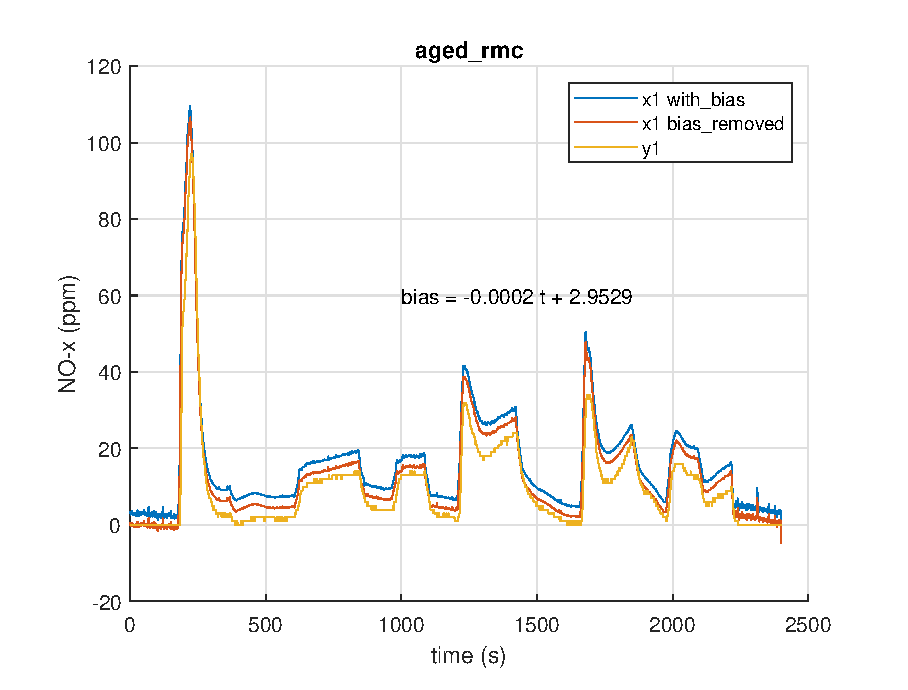
\includegraphics[width=\textwidth]{./figs/chi_est/aged_rmc_NOx_bias.eps}
        \end{figure}
    \end{minipage}
    \begin{minipage}{0.49\textwidth}
        \begin{figure}[H]
            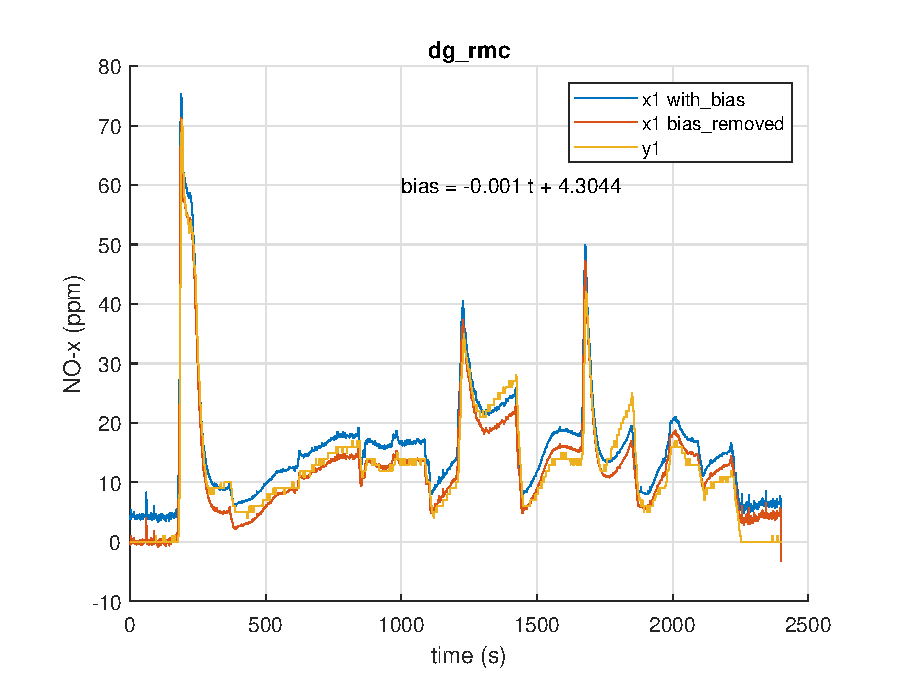
\includegraphics[width=\textwidth]{./figs/chi_est/dg_rmc_NOx_bias.eps}
        \end{figure}
    \end{minipage}
        \caption{Sensor bias correction for RMC cycles}
\end{figure}



\subsection{Effect of $NH_3$ sensor bias and minimum threshold for cross-sensitivity}

The ammonia sensor used for ammonia measurement also has bias and there is a
threshold on ammonia for which the $NO_x$ sensor becomes cross-sensitive to
ammonia. Thus the expression for cross-sensitivity becomes:

\begin{align*}
    y_1 &= \lr{x_1 - b_0} + \chi (x_2 - b_{th})\\
\end{align*}

\subsection{Least-squares estimation assuming temperature independence}
\itbf{Assumption}: The temperature changes in RMC cycle don't effect the
cross-sensitivity factor significantly. Thus, it can be treated as a constant
w.r.t temperature fluctuations in that range.

We have,
\begin{align*}
    \underbrace{y_1 - x_1}_{\pmb y} &= \underbrace{\bm{x_2 & -1}}_{\pmb \phi^T} \underbrace{\bm{ \chi \\ \underbrace{\chi b_{th} + b_0}_{=b}}}_{ \pmb \theta}\\
\end{align*}

\begin{figure}[H]
    \begin{minipage}{0.49\textwidth}
        \begin{figure}[H]
            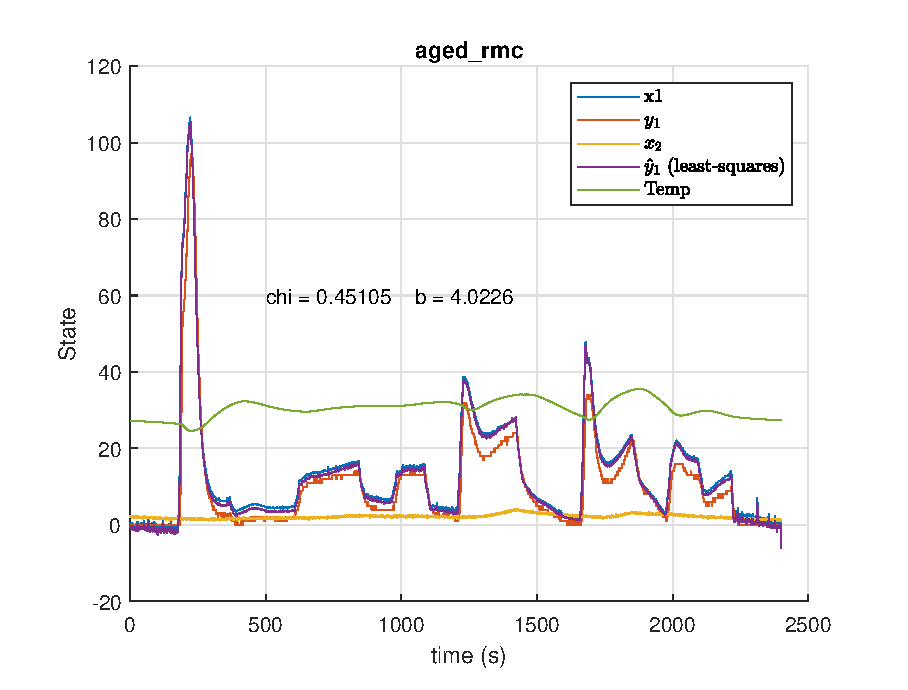
\includegraphics[width=\textwidth]{./figs/chi_est/aged_rmc_chi.eps}
        \end{figure}
    \end{minipage}
    \begin{minipage}{0.49\textwidth}
        \begin{figure}[H]
            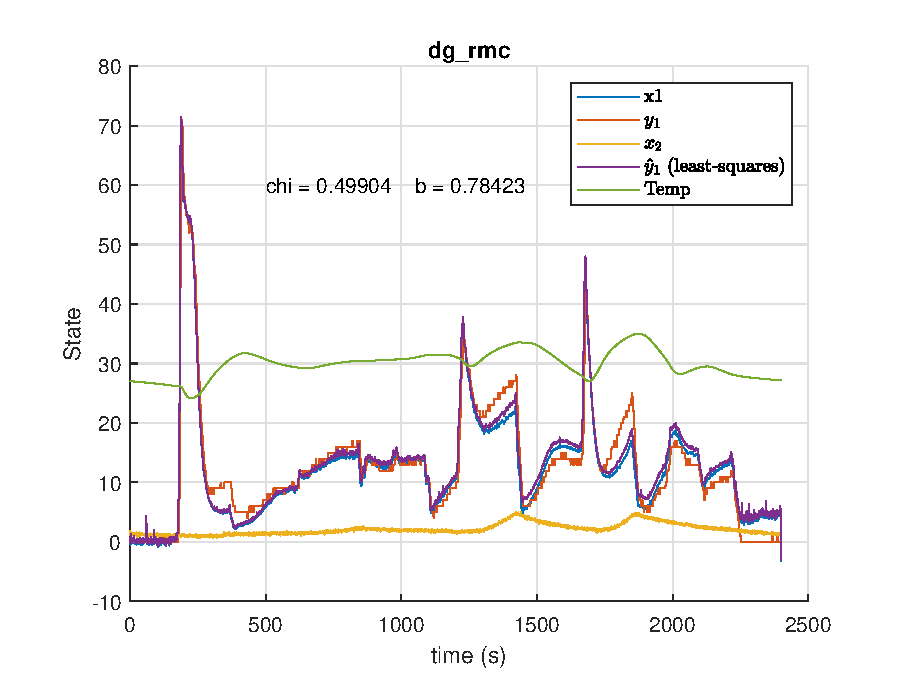
\includegraphics[width=\textwidth]{./figs/chi_est/dg_rmc_chi.eps}
        \end{figure}
    \end{minipage}
        \caption{$\chi$ estimation for rmc cycles}
\end{figure}

\begin{figure}[H]
    \centering
    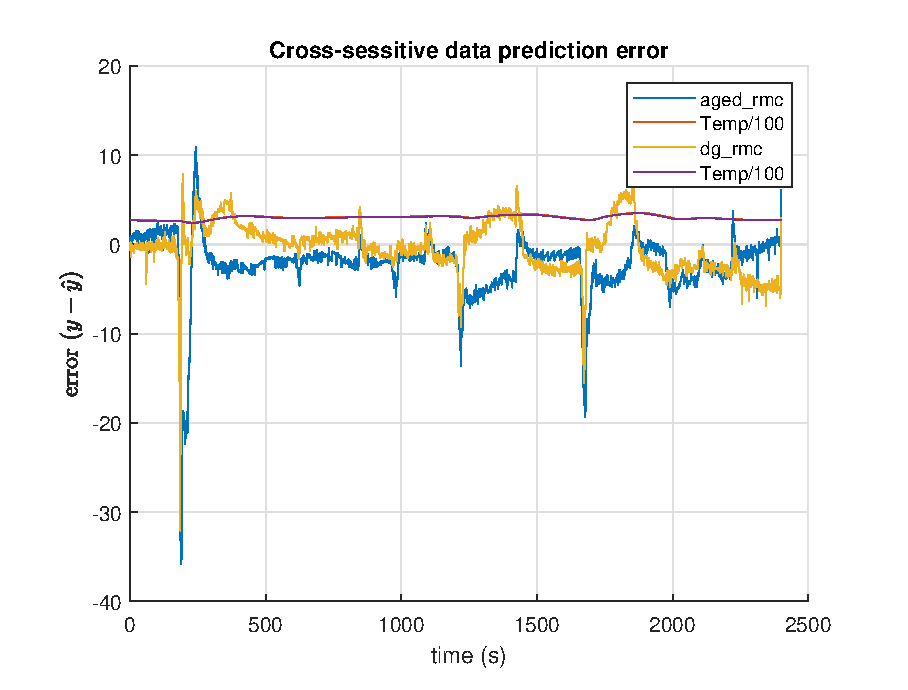
\includegraphics[width = 0.5 \textwidth]{./figs/chi_est/chi_error.eps}
    \caption{Error in $\chi$ estimation}
\end{figure}

The error can be reduced by introducing the effects of temperature into $\chi$.


\subsection{$\chi$ as a temperature function}
For simplicity, $\chi$ is assumed to be a linear function of temperature.
\begin{align*}
    \chi(T) &= a T - b_T
\end{align*}

\subsection{Least-squares estimation with temperature dependence}
Assuming the sensor-bias is not time-varying ($\because$ $b_1$ is small). The
sensor bias, cross-sensitivity threshold and temperature dependence can be
combined into:

\begin{align*}
    y_1 &=  \lr{x_1 - b_0} + \lr{aT - b_{T}} \lr{x_2 - b_{th}}\\
    \lr{y_1 - x_1} &= a T x_2 - a b_{th} T - b_{T} x_2 + (b_T b_{th} - b_0)\\
    \underbrace{y_1 - x_1}_{\pmb y} &= \underbrace{\bm{T x_2 & -T & -x_2 & 1}}_{\pmb \phi^T} \underbrace{\bm{a \\ a b_{th} \\ b_T \\ b_T b_{th} - b_0}}_{\pmb \theta}\\
\end{align*}

\begin{figure}[H]
    \begin{minipage}{0.49\textwidth}
        \begin{figure}[H]
            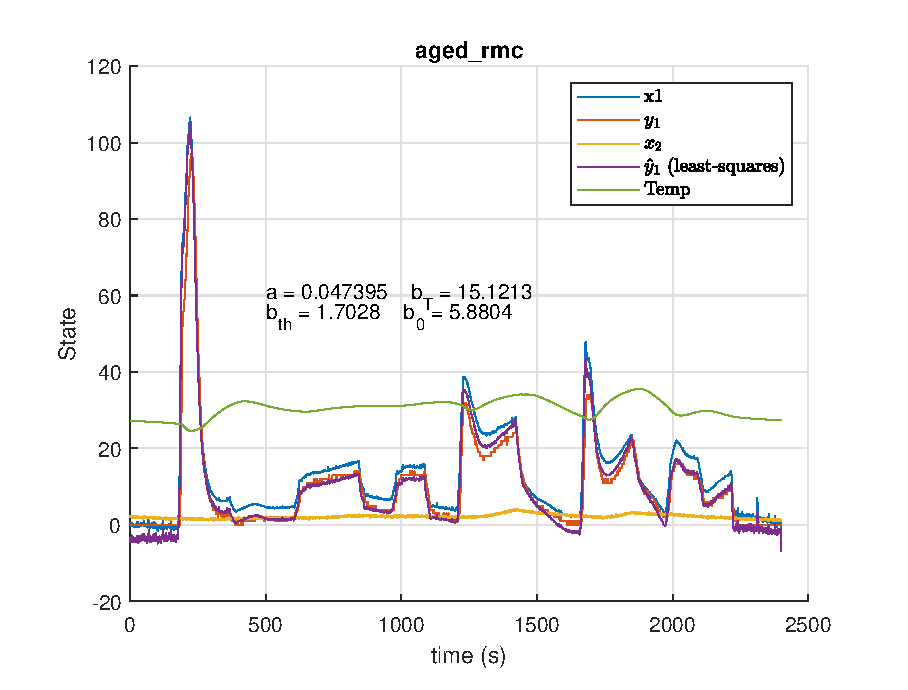
\includegraphics[width=\textwidth]{./figs/chi_est/aged_rmc_chiT.eps}
        \end{figure}
    \end{minipage}
    \begin{minipage}{0.49\textwidth}
        \begin{figure}[H]
            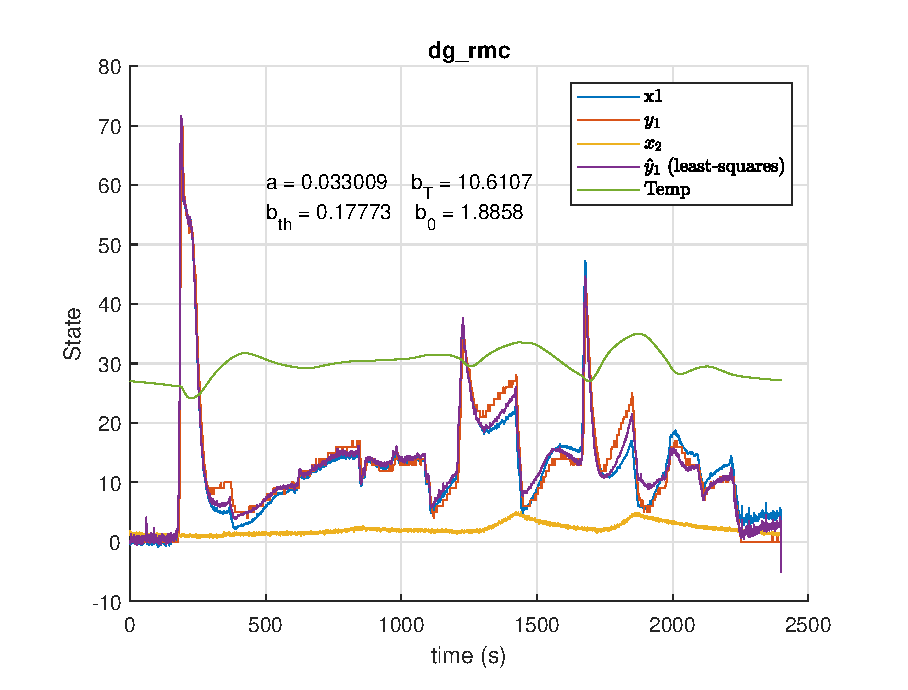
\includegraphics[width=\textwidth]{./figs/chi_est/dg_rmc_chiT.eps}
        \end{figure}
    \end{minipage}
        \caption{$\chi$ estimation for rmc cycles}
\end{figure}

\begin{figure}[H]
    \begin{minipage}{0.49\textwidth}
        \begin{figure}[H]
            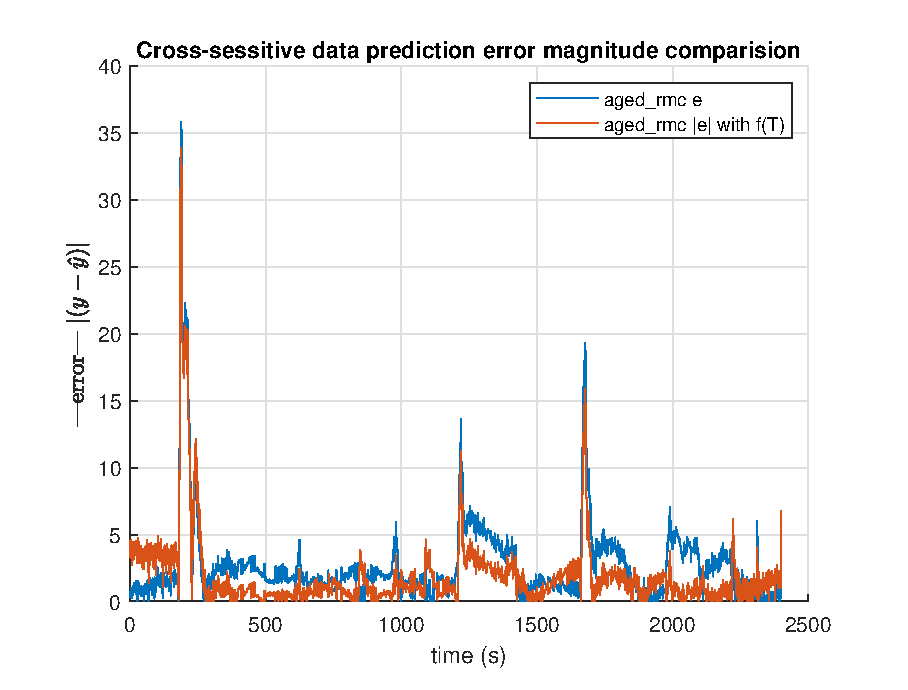
\includegraphics[width=\textwidth]{./figs/chi_est/aged_error_comp.eps}
        \end{figure}
    \end{minipage}
    \begin{minipage}{0.49\textwidth}
        \begin{figure}[H]
            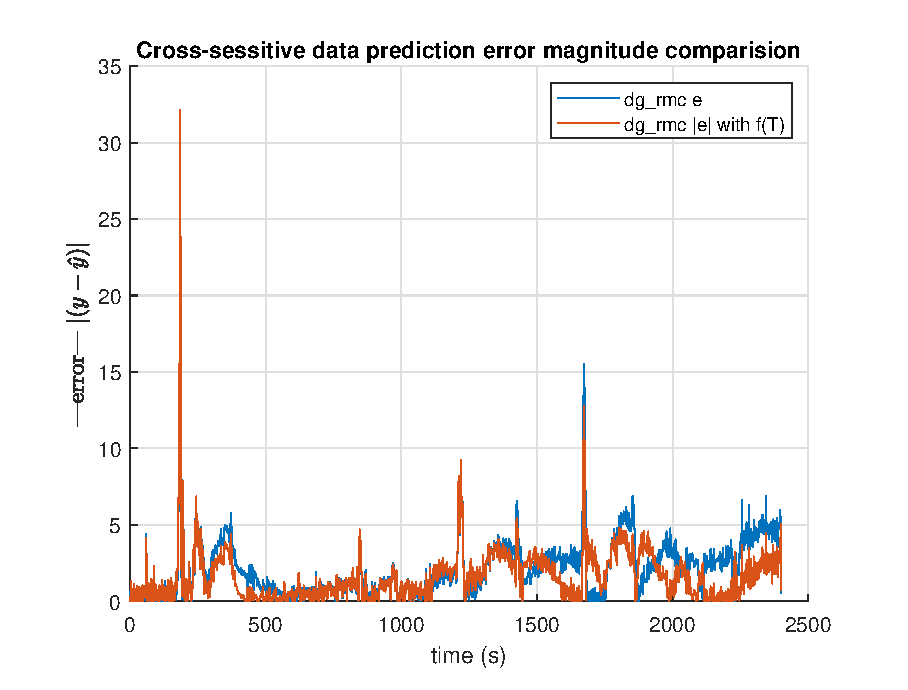
\includegraphics[width=\textwidth]{./figs/chi_est/dg_error_comp.eps}
        \end{figure}
    \end{minipage}
        \caption{Effect of temperature on prediction errors for $\chi$ estimation in RMC cycles}
\end{figure}


Introducing temperature clearly decreased the prediction error in the model. However, the reduction in error, while noticeable, is not significant when compared to the temperature-independent model, whose error remains within acceptable limits.

% ==============================================================================
\newpage
\section{Appencix}
\subsection{4 State Dynamic Model}
A four state nonlinear model for the above reactions can be developed using
Arrhenius equations, CSTR assumption and further simplification based on the
following assumptions:

\subsection{Assumptions}
\begin{enumerate}
    \item Slow SCR reaction is neglected.
    \begin{itemize}
        \item The flow rate of the exhaust would ensure that the not a significant concentration of tail-pipe exhaust components are due to the slow SCR reaction \cite{nova2014urea}.
    \end{itemize}

    \item Mass transfer is neglected. That means the chemical kinetics in the catalyst are reaction controlled.
    \begin{itemize}
        \item The standard SCR reaction rate is faster than the flow rate of the exhaust fluids.
    \end{itemize}

    \item Nitrogen selectivity for ammonia oxidation is $100\%$.
    \begin{itemize}
        \item This assumption is relaxed by including algebraic relationship between selectivity and the temperature (ASC model \cite{jain2023diagnostics}).
    \end{itemize}

    \item Reaction rates are assumed to be a function of the gas phase concentration of $NO_x$ and ammonia storage.
\end{enumerate}

\subsubsection{Additional Reaction Rates}
\begin{enumerate}
\item Fast SCR Reaction (\ref{eqn::fast_scr}):
$ R_2 = k_2 \exp\lr{-\frac{E_2}{RT}} C_{NO} C_{N_2O} \theta \Theta V^2 $
\item NO oxidation (\ref{eqn::NOX}):
$ R_5 = \underbrace{k_5 \exp \lr{- \frac{E_5}{RT}}}_{r_5} C_{NO} C_{O_2} V^2 $
\end{enumerate}

\subsubsection{Dynamic model}
Using above assumptions and definitions, we have the dynamic model \cite{nova2014urea}:
\begin{equation} \label{eqn::4_state}
    \bm{\dot C_{NO} \\
        \dot C_{NO_2}\\
        \dot C_{NH_3}\\
        \dot \theta_{NH_3}\\
        } =
    \bm{
        -r_1 C_{NO} C_{O_2} \theta_{NH_3} \Theta V
        - 0.5 r_2 C_{NO} C_{NO_2} \theta_{NH_3} \Theta V
        -r_5 C_{NO} C_{O_2} V
        -b C_{NO}\\
        %===
        -0.5 r_2 C_{NO} C_{NO_2} \theta_{NH_3} \Theta V
        + r_5 C_{NO} C_{O_2} V
        -b C_{NO_2}\\
        %===
        -C_{NH_3} \lrb{\Theta r_{rF} \lr{1 - \theta_{NH_3}} + b} + V^{-1} r_{4R} \Theta \theta_{NH_3}\\
        %===
        -\theta_{NH_3} \lr{r_{4F}C_{NH_3} V + r_3 C_{O_2}V + r_{4R} + r_1 C_{NO} C_{O_2} V^2 + r_2 C_{NO} C_{NO_2} V^2} + r_{4F} C_{NH_3} V
    }
    + b \bm{C_{NO, in} \\ C_{NO_2, in} \\ C_{NH_3} \\ 0}
\end{equation}
Where,
\begin{align*}
    b = \frac{F}{V}
\end{align*}

\subsubsection{Previously used 3-state dynamic model}
The 3-state dynamic model used previously \cite{jain2023diagnostics} is as follows:
\begin{figure}[H]
    \begin{minipage}{0.59\textwidth}
        \begin{align*}
        &\text{\itbf{Dynamics}:}\\
            \dot x_1 &= \lr{\frac{F}{V}} \lr{u_1 - x_1} - K \alpha_{ads} x_1 (1 - x_3) + K \alpha_{des} x_3\\
            %===
            \dot x_2 &= \lr{\frac{F}{V}} \lr{u_2 - x_2} - K \alpha_{SCR} x_2 x_3\\
            %===
            \dot x_3 &= \alpha_{ads} x_1 \lr{ 1 - x_3} - \alpha_{SCR} x_2 x_3 - \alpha_{des} x_3 - \alpha_{oxi} x_3
        \end{align*}
    \end{minipage}
    \begin{minipage}{0.4\textwidth}
        \begin{align*}
            &\\
            \dot u_1 &= \frac{1}{\tau} \lr{ -u_1 +\eta_{urea} u_{1, ideal}} & [\text{actuator dynamics}]\\
            %===
            K &= \frac{S_1}{V} \exp\lr{-S_2 T}\\
            %===
            \alpha_i &= A_i \exp\lr{-\frac{E_i}{RT}}
            %===
            & i = ads, des, SCR, oxi
        \end{align*}
    \end{minipage}
    \begin{minipage}{\textwidth}
        \begin{align*}
            \text{\itbf{States}:}&\\
            %===
            x_1 &- NH_3 \text{ concentration at SCR-out } \lr{mol/m^3}\\
            %===
            x_2 &- NO_x \, (NO) \text{ concentration at SCR-out } \lr{mol/m^3}\\
            %===
            x_3 &- NH_3 \text{ storage capacity fraction in SCR } = \frac{\text{Moles of $NH_3$ adsorbed}}{\text{Total moles of $NH_3$ that can be adsorbed}}\\
            %===
            \text{\itbf{Inputs}:}&\\
            %===
            u_1 &- NH_3 \text{ injected concentration at SCR-in } \lr{mol/m^3}\\
            &\qquad \begin{matrix*}[l]
                \eta_{urea} &-& \text{urea} \rightarrow NH_3 \text{ conversion efficiency}\\
                 \tau &-& \text{urea} \rightarrow NH_3 \text{ time-constant}\\
                 u_{1, ideal} &-& \text{ideal $u_1$ if $\eta_{urea} = 1$ (constant parameter obtained through calibration)}\\
            \end{matrix*}\\
            %===
            u_2 &- NO_x (NO) \text{ concentration at SCR-in } \lr{mol/m^3}\\
            %===
            \text{\itbf{Parameters}:}&\\
            K &- \text{SCR catalyst's } NH_3 \text{ storage capacity } \lr{mols}\\
            &\qquad \begin{matrix*}[l]
                S_1, S_2 &-& \text{Aging parameters of the catalyst}
            \end{matrix*}\\
            F &- \text{Exhaust gas volume flow rate } \lr{m^3/s}\\
            V &- \text{Volume of the catalyst } \lr{m^3}\\
            \alpha_i &- \text{Reaction rate of $i^{th}$ reaction}\\
            &\qquad \begin{matrix*}[l]
            E_i &-& \text{Activation Energy of $i^{th}$ reaction}\\
            A_i &-& \text{Pre-exponential factor of $i^{th}$ reaction}\\
            i : SCR &-& \text{Standard SCR reaction}\\
            i : ads &-& NH_3 \text{ adsorption}\\
            i : des &-& NH_3 \text{ desorption}\\
            i : oxi &-& NH_3 \text{ oxidation}
            \end{matrix*}
                   \end{align*}
    \end{minipage}
\end{figure}

\newpage
\nocite{}
\bibliographystyle{unsrt}
\bibliography{refs}

\end{document}
